\chapter{Experimental results} \label{chap:experimental_results}

This chapter presents the results of our experiments. Specifically, we compare the performance of three optimization algorithms:
\begin{itemize}
    \item \textit{genetic algorithm (GA)},
    \item \textit{hill climbing (HC)},
    \item \textit{simulated annealing (SA)},
\end{itemize}
on datasets B, C, D, E, and F.
Section~\ref{sec:experimental_setup} explains the setup of the experiments and format of the results shown in the figures and tables. The following sections present the results for each dataset, including plots and tables summarizing the performance of each algorithm. The datasets are presented in ascending order of their size (see Section~\ref{sec:datasets} for more details).

\section{Experimental setup} \label{sec:experimental_setup}

As previously mentioned, Tables~\ref{tab:hyperparams_shared} and \ref{tab:hyperparams_datasets_specific} summarize the hyperparameters used for each algorithm and dataset. The experiments were performed on either AMD EPYC 9454 or AMD EPYC 9474F CPUs. Each setting was run with 10 different fixed seeds, and the results were averaged to ensure reliability. As explained in Section~\ref{sec:hyperparameter_search}, all three algorithms were run for the same fixed budget of fitness evaluations.

Note that comparing by number of evaluations is somewhat disadvantageous for the genetic algorithm, which inherently performs a broader search of the state space. Additionally, fitness evaluations within each population are computed in parallel, which can result in significantly faster runtimes compared to single-state methods. Nevertheless, we chose the number of fitness evaluations as the comparison metric instead of runtime, as it better reflects algorithmic efficiency and is independent of implementation details and the specific hardware used.

For each dataset, we provide a plot illustrating the performance of all three methods throughout the optimization process. The x-axis indicates the number of fitness evaluations, while the primary y-axis shows the normalized score (see Section~\ref{subsec:score_normalization}).
For completeness, the secondary y-axis displays the absolute score.
For genetic algorithm, the plotted curve represents the best score within the current population. For hill climbing and simulated annealing, the curve shows the current score at each step.  All curves are averaged over 10 runs, with the shaded areas indicating the standard deviation.

For each dataset, we also include a table reporting the overall best score achieved by each algorithm, averaged over 10 runs, along with the total runtime. The runtime is included to give a general idea of how long each method took to run, but it should not be interpreted as an exact metric.

Finally, we summarize in Table~\ref{tab:best_scores} the best scores achieved by each algorithm in a single run (out of 10 seeds), and compare them to the maximum known score for each dataset. The schedules corresponding to the best score for each dataset are included in the thesis attachment.

\newpage
\section{Dataset E} \label{sec:dataset_e}

For dataset E, the smallest optimized dataset, \textit{SA} not only outperformed \textit{GA} and \textit{HC}, but even exceeded the best known score, which explains why its normalized score in Table~\ref{tab:dataset_e_results} is greater than 1. While \textit{GA} and \textit{HC} quickly reached good scores above 80\% of the best known score, they converged early and improved only slightly afterwards. In contrast, \textit{SA} started off slower and volatile, but continued to steadily improve its score throughout the optimization process (see Figure~\ref{fig:dataset_e_experiment}).

\bigskip

\begin{figure}[h]
    \centering
    % 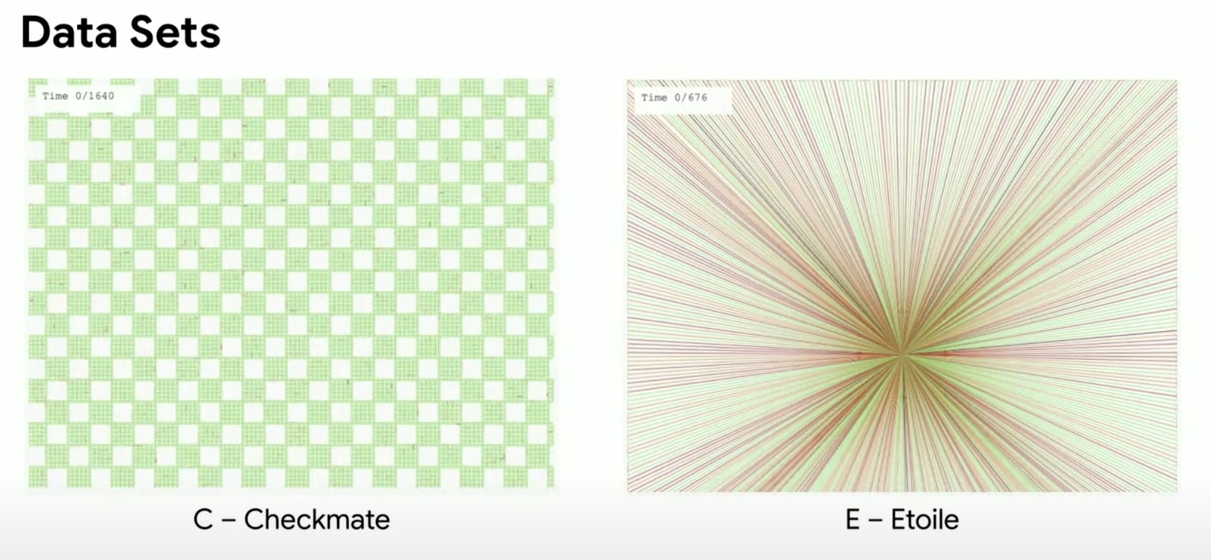
\includegraphics[width=\linewidth]{img/screenshots/hashcode_datasets_c_e.png}
    % 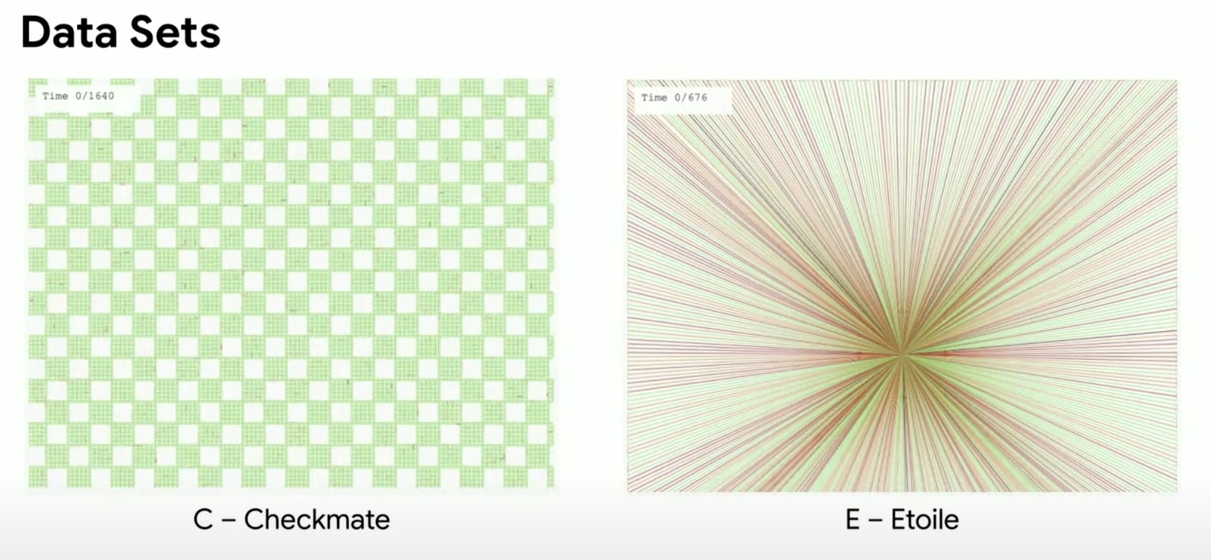
\includegraphics[width=.8\linewidth]{img/screenshots/hashcode_datasets_c_e.png}
    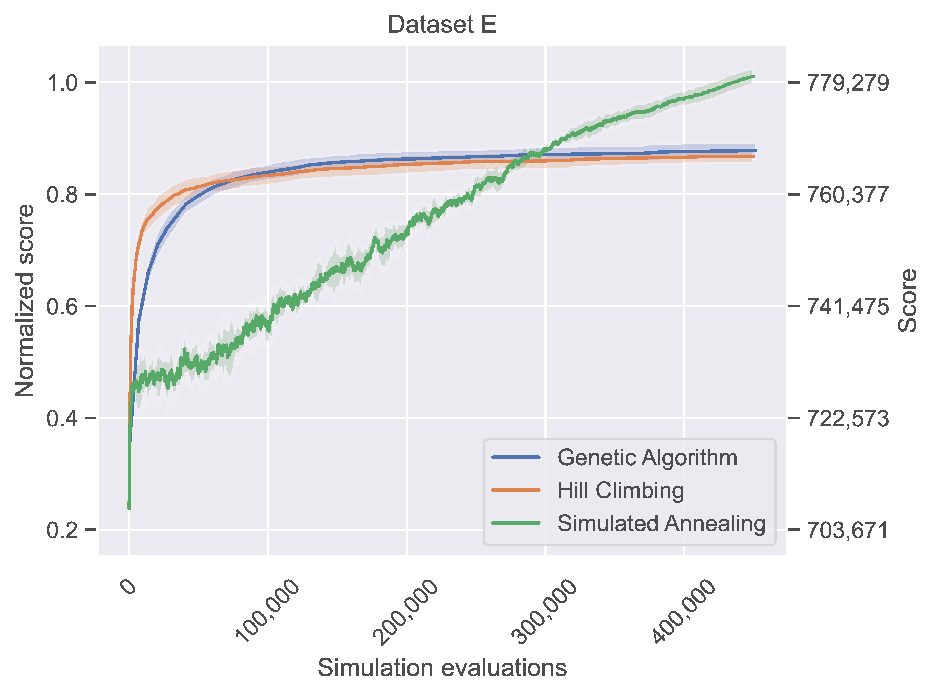
\includegraphics[width=\linewidth]{img/experiments/pdfa-e_Genetic Algorithm_Hill Climbing_Simulated Annealing.pdf}
    \caption[Performance of the algorithms on dataset E]{
        Performance of the algorithms on dataset E.
    }
    \label{fig:dataset_e_experiment}
\end{figure}

\bigskip

\begin{table}[h]
\centering\footnotesize\sf
\begin{tabular}{lccc}
\toprule
& Normalized Score & Score & Runtime (mm:ss) \\
\midrule
\textcolor{myblue}{\textbf{Genetic Algorithm}} & 0.88 & 767,768 & \textbf{06:58} \\
\textcolor{myorange}{\textbf{Hill Climbing}} & 0.87 & 766,798 & 07:03 \\
\textcolor{mygreen}{\textbf{Simulated Annealing}} & \textbf{1.01} & \textbf{780,299} & 07:10 \\
\bottomrule
\end{tabular}
\caption[Statistics for dataset E]{
    Final statistics for dataset E.
}
\label{tab:dataset_e_results}
\end{table}

\newpage
\section{Dataset B} \label{sec:dataset_b}

For dataset B, \textit{SA} again achieved the best score among the three algorithms. This time, it performed the best since the very beginning of the optimization process (see Figure~\ref{fig:dataset_b_experiment}). Although close, it fell short of the best known score, reaching 97\% of it (see Table~\ref{tab:dataset_b_results}). \textit{HC} started off similarly to \textit{SA}, but again converged early and ultimately performed the worst---though it still achieved a good score. \textit{GA} performed noticeably better than \textit{HC} but did not reach the performance of \textit{SA}. Note that the parallel fitness evaluation in \textit{GA} starts to show its advantage, with the \textit{GA} runtime being approximately one-third shorter than the other two algorithms (see Table~\ref{tab:dataset_b_results}).

\bigskip

\begin{figure}[h]
    \centering
    % 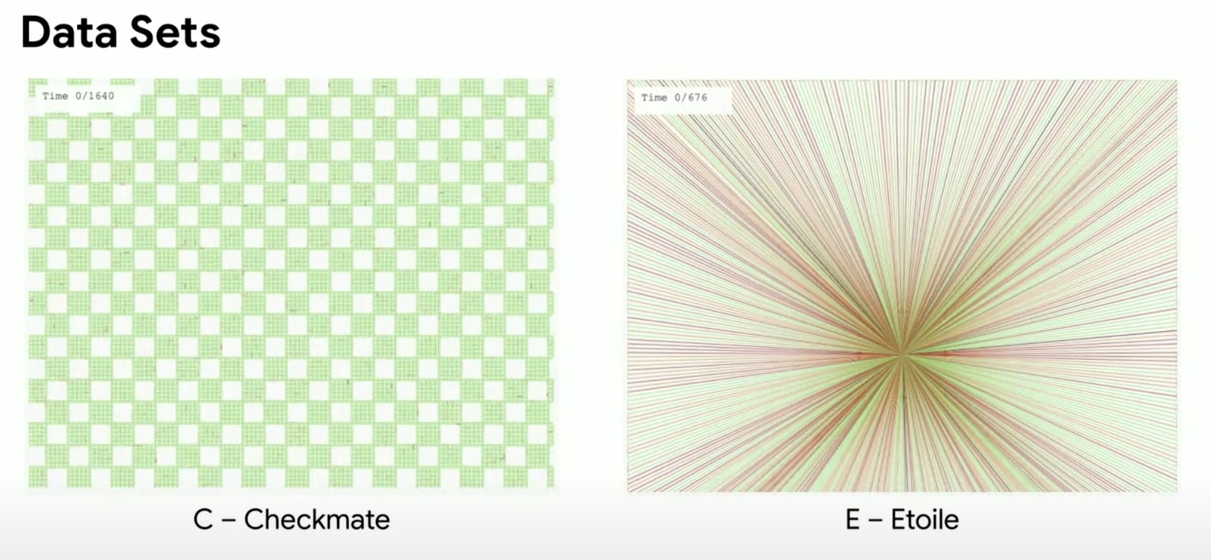
\includegraphics[width=\linewidth]{img/screenshots/hashcode_datasets_c_e.png}
    % 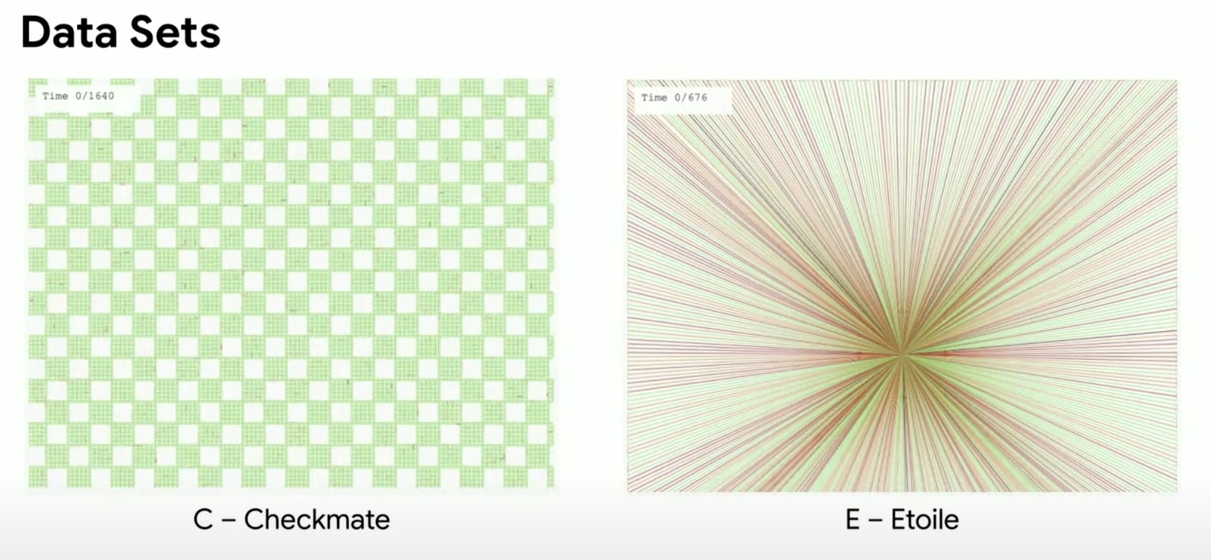
\includegraphics[width=.8\linewidth]{img/screenshots/hashcode_datasets_c_e.png}
    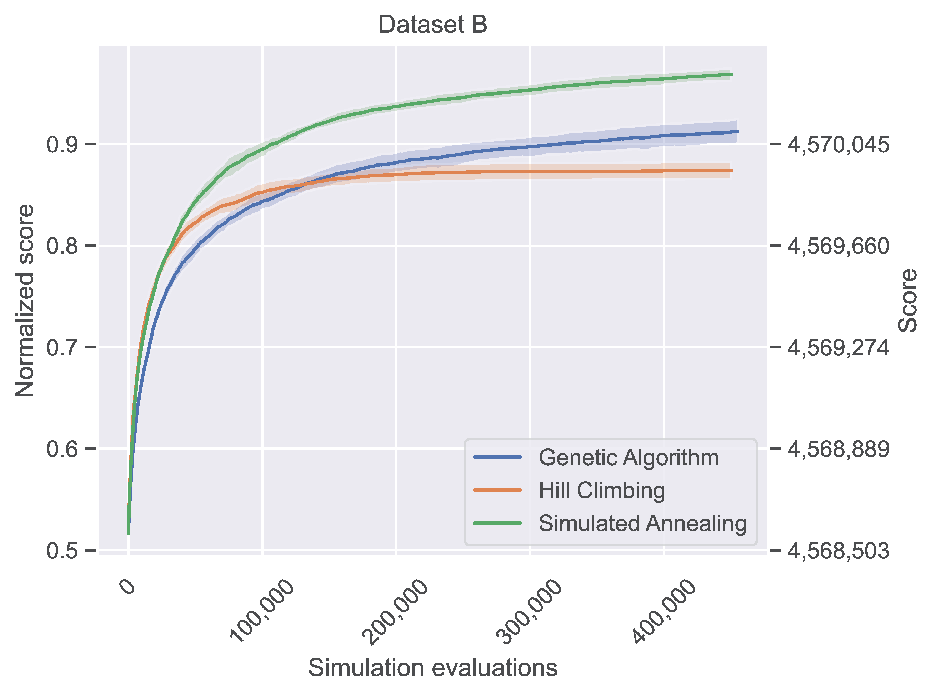
\includegraphics[width=\linewidth]{img/experiments/pdfa-b_Genetic Algorithm_Hill Climbing_Simulated Annealing.pdf}
    \caption[Performance of the algorithms on dataset B]{
        Performance of the algorithms on dataset B.
    }
    \label{fig:dataset_b_experiment}
\end{figure}

\bigskip

\begin{table}[h]
\centering\footnotesize\sf
\begin{tabular}{lccc}
\toprule
& Normalized Score & Score & Runtime (h:mm:ss) \\
\midrule
\textcolor{myblue}{\textbf{Genetic Algorithm}} & 0.91 & 4,570,095 & \textbf{0:42:29} \\
\textcolor{myorange}{\textbf{Hill Climbing}} & 0.87 & 4,569,945 & 1:00:08 \\
\textcolor{mygreen}{\textbf{Simulated Annealing}} & \textbf{0.97} & \textbf{4,570,309} & 0:59:07 \\
\bottomrule
\end{tabular}
\caption[Statistics for dataset B]{
    Final statistics for dataset B.
}
\label{tab:dataset_b_results}
\end{table}

\newpage
\section{Dataset F} \label{sec:dataset_f}

For dataset F, the performance of all three algorithms is much closer than in previous datasets, due to starting from a really good initial solution. Nonetheless, \textit{SA} achieved the highest score, \textit{HC} performed the worst, and \textit{GA} was in between (see Table~\ref{tab:dataset_f_results}). As shown in Figure~\ref{fig:dataset_f_experiment}, the shaded areas representing standard deviation overlap quite a lot, indicating that there is not a big difference between the algorithms. \textit{GA} again demonstrated a significantly shorter runtime.

\bigskip

\begin{figure}[h]
    \centering
    % 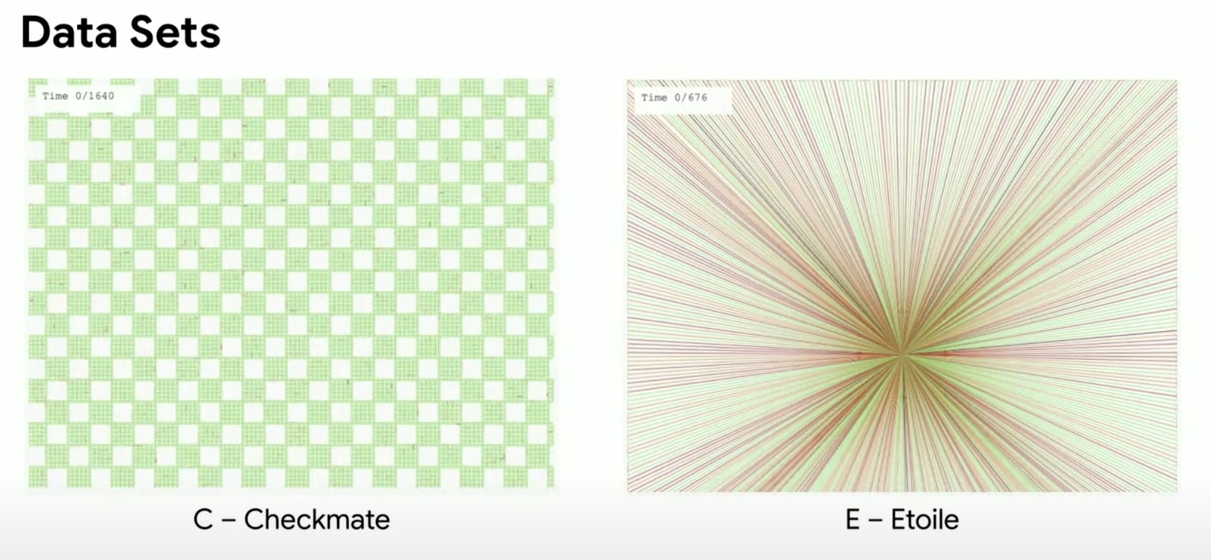
\includegraphics[width=\linewidth]{img/screenshots/hashcode_datasets_c_e.png}
    % 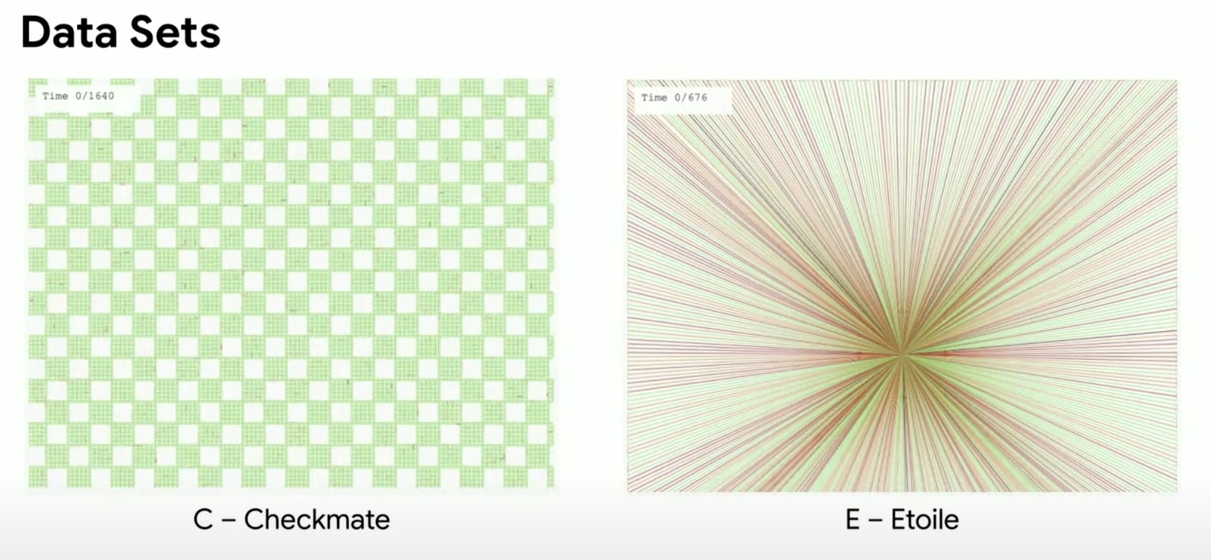
\includegraphics[width=.8\linewidth]{img/screenshots/hashcode_datasets_c_e.png}
    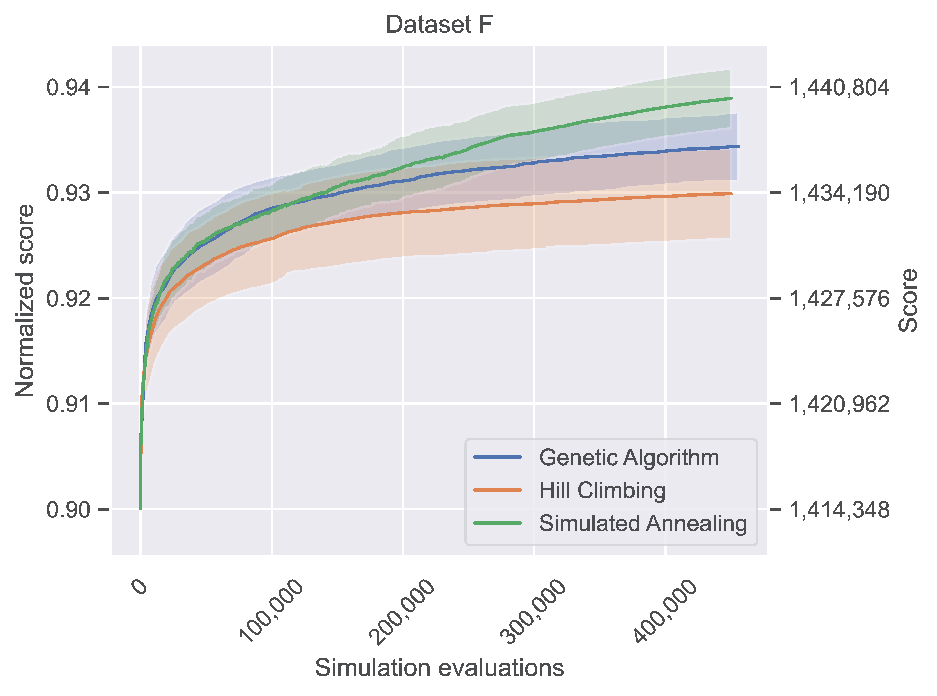
\includegraphics[width=\linewidth]{img/experiments/pdfa-f_Genetic Algorithm_Hill Climbing_Simulated Annealing.pdf}
    \caption[Performance of the algorithms on dataset F]{
        Performance of the algorithms on dataset F.
    }
    \label{fig:dataset_f_experiment}
\end{figure}

\bigskip

\begin{table}[h]
\centering\footnotesize\sf
\begin{tabular}{lccc}
\toprule
& Normalized Score & Score & Runtime (h:mm:ss) \\
\midrule
\textcolor{myblue}{\textbf{Genetic Algorithm}} & 0.93 & 1,437,086 & \textbf{1:48:33} \\
\textcolor{myorange}{\textbf{Hill Climbing}} & 0.93 & 1,434,129 & 2:41:04 \\
\textcolor{mygreen}{\textbf{Simulated Annealing}} & \textbf{0.94} & \textbf{1,440,097} & 2:28:03 \\
\bottomrule
\end{tabular}
\caption[Statistics for dataset F]{
    Final statistics for dataset F.
}
\label{tab:dataset_f_results}
\end{table}

\newpage
\section{Dataset C} \label{sec:dataset_c}

For dataset C, the curves shown in Figure~\ref{fig:dataset_c_experiment} resemble those observed for dataset B (see Figure~\ref{fig:dataset_b_experiment}). \textit{SA} consistently outperformed the other algorithms from the start and again exceeded the best known score, with the normalized score above 1 (see Table~\ref{tab:dataset_c_results}). \textit{GA} and \textit{HC} performed similarly, with \textit{GA} narrowly outperforming \textit{HC}. As in previous datasets, \textit{GA} finished in a significantly shorter time (see Table~\ref{tab:dataset_c_results}).

\bigskip

\begin{figure}[h]
    \centering
    % 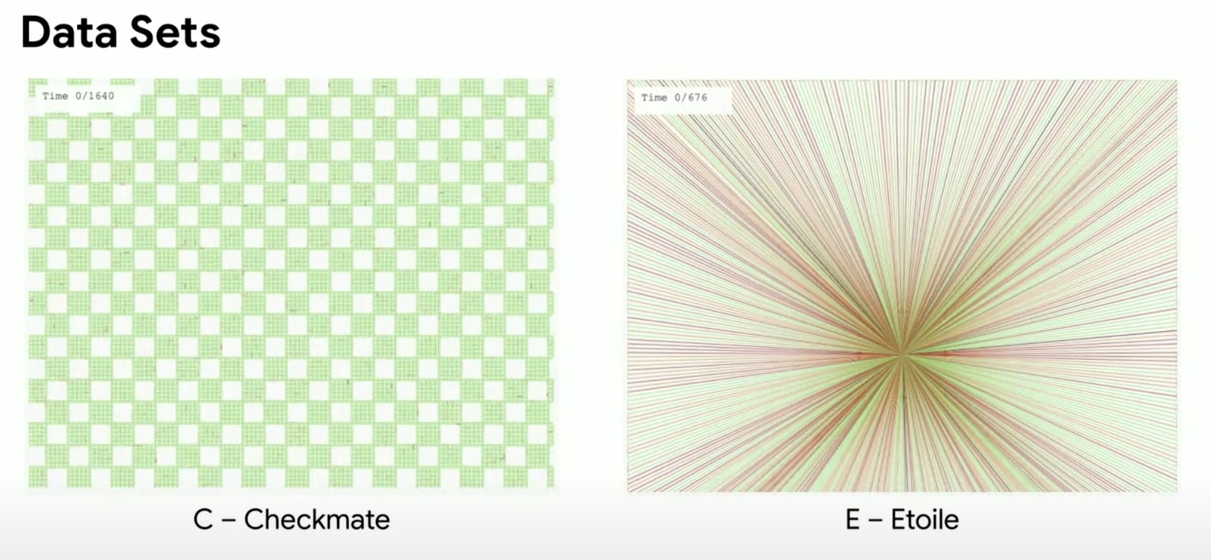
\includegraphics[width=\linewidth]{img/screenshots/hashcode_datasets_c_e.png}
    % 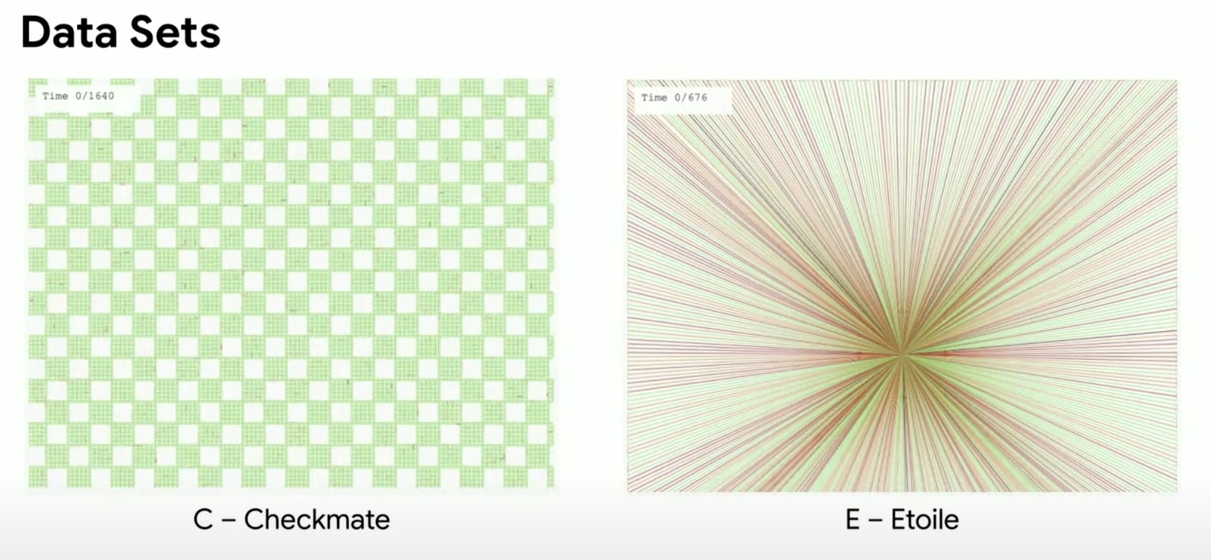
\includegraphics[width=.8\linewidth]{img/screenshots/hashcode_datasets_c_e.png}
    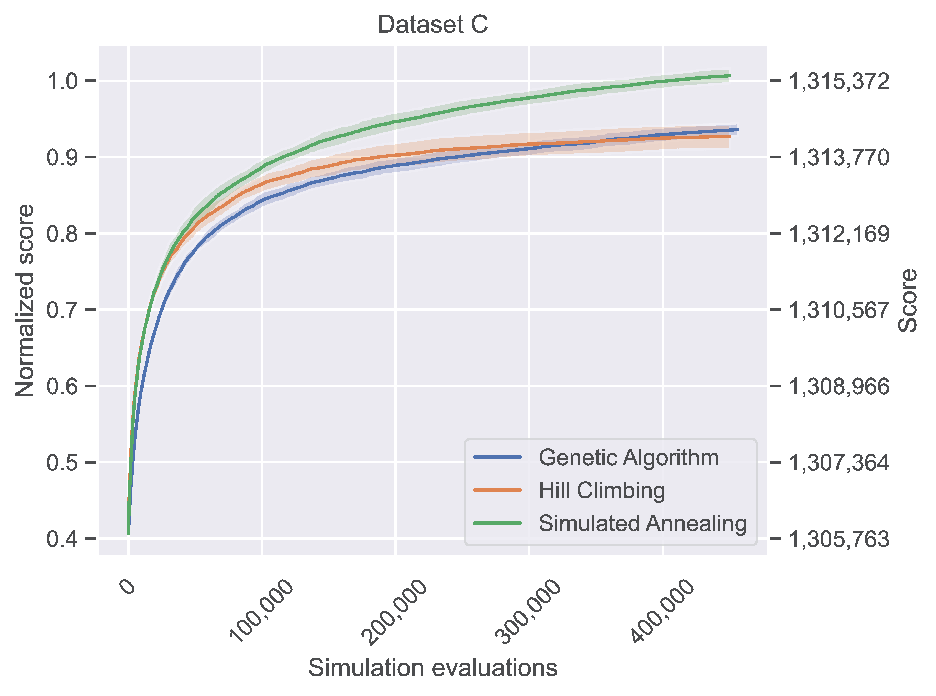
\includegraphics[width=\linewidth]{img/experiments/pdfa-c_Genetic Algorithm_Hill Climbing_Simulated Annealing.pdf}
    \caption[Performance of the algorithms on dataset C]{
        Performance of the algorithms on dataset C.
    }
    \label{fig:dataset_c_experiment}
\end{figure}

\bigskip

\begin{table}[h]
\centering\footnotesize\sf
\begin{tabular}{lccc}
\toprule
& Normalized Score & Score & Runtime (h:mm:ss) \\
\midrule
\textcolor{myblue}{\textbf{Genetic Algorithm}} & 0.94 & 1,314,347 & \textbf{2:02:52} \\
\textcolor{myorange}{\textbf{Hill Climbing}} & 0.93 & 1,314,200 & 3:33:10 \\
\textcolor{mygreen}{\textbf{Simulated Annealing}} & \textbf{1.01} & \textbf{1,315,476} & 3:26:31 \\
\bottomrule
\end{tabular}
\caption[Statistics for dataset C]{
    Final statistics for dataset C.
}
\label{tab:dataset_c_results}
\end{table}

\newpage
\section{Dataset D} \label{sec:dataset_d}

For dataset D, the largest dataset by far, the results are different from all previous datasets. \textit{HC}, the weakest algorithm in the previous cases, performed the best here, although only slightly ahead of \textit{SA} (see Figure~\ref{fig:dataset_d_experiment}). It is likely that the algorithms would have benefited from running for more evaluations, as their performance curves had not yet fully converged.
\textit{GA}, in particular, performed the worst here, but completed in less than half the time of the other two algorithms (see Table~\ref{tab:dataset_d_results}), fully utilizing its parallel evaluation.
However, the runtimes for this dataset were already much longer than for the rest of the datasets combined, showing how large and demanding dataset D really was.

\bigskip

\begin{figure}[h]
    \centering
    % 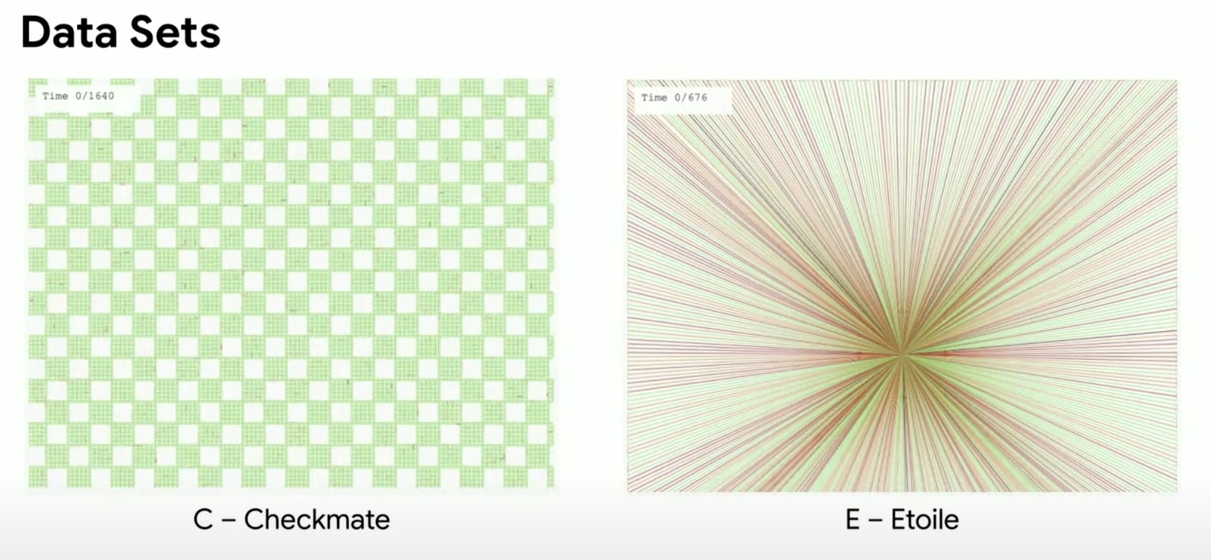
\includegraphics[width=\linewidth]{img/screenshots/hashcode_datasets_c_e.png}
    % 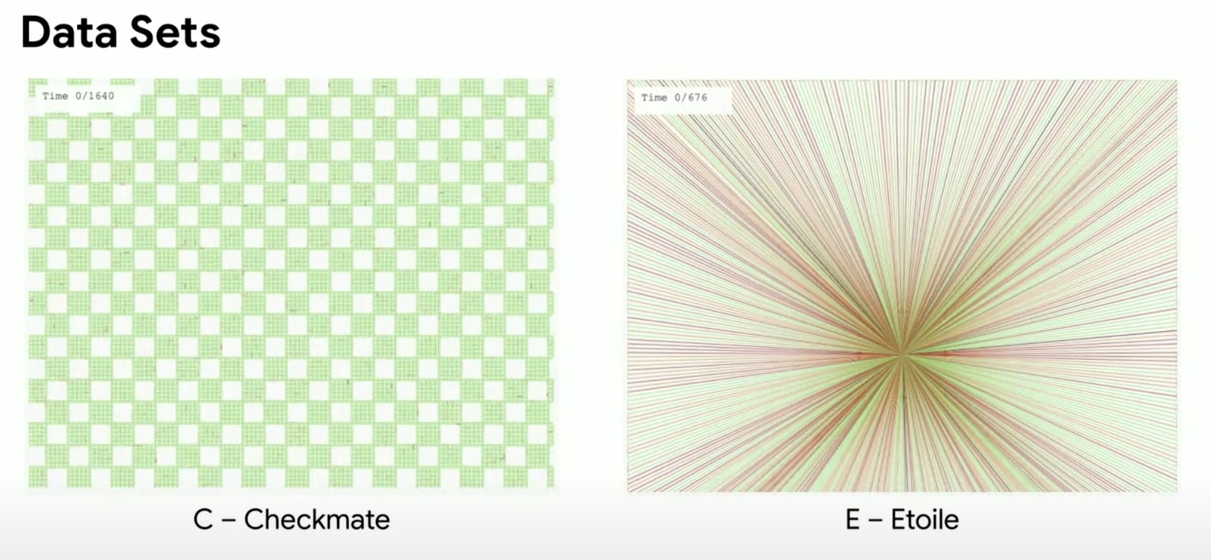
\includegraphics[width=.8\linewidth]{img/screenshots/hashcode_datasets_c_e.png}
    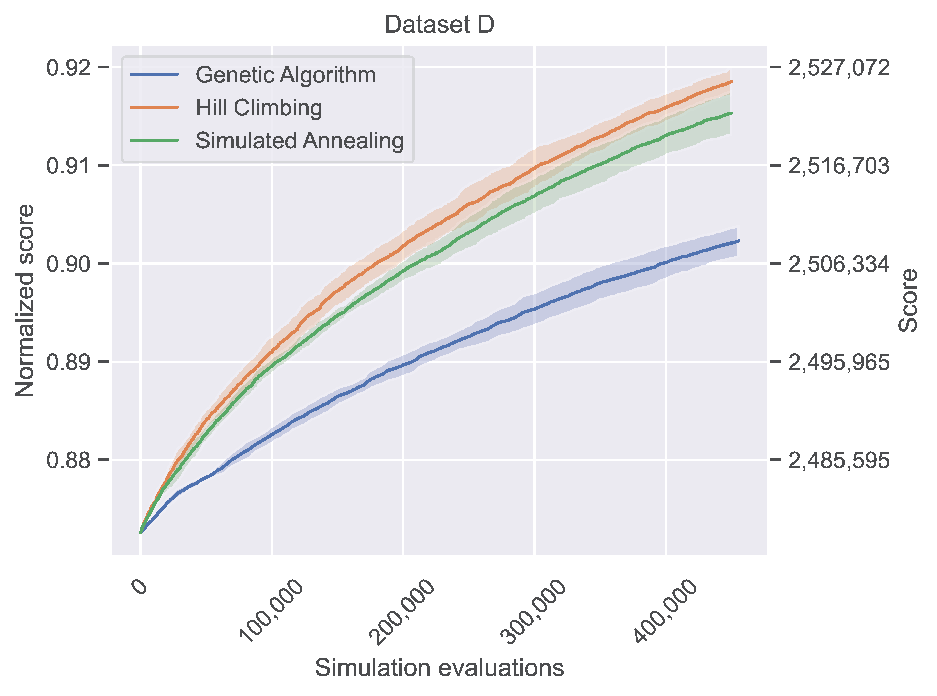
\includegraphics[width=\linewidth]{img/experiments/pdfa-d_Genetic Algorithm_Hill Climbing_Simulated Annealing.pdf}
    \caption[Performance of the algorithms on dataset D]{
        Performance of the algorithms on dataset D.
    }
    \label{fig:dataset_d_experiment}
\end{figure}

\bigskip

\begin{table}[h]
\centering\footnotesize\sf
\begin{tabular}{lccc}
\toprule
& Normalized Score & Score & Runtime (hh:mm:ss) \\
\midrule
\textcolor{myblue}{\textbf{Genetic Algorithm}} & 0.90 & 2,508,730 & \textbf{09:41:52} \\
\textcolor{myorange}{\textbf{Hill Climbing}} & \textbf{0.92} & \textbf{2,525,531} & 20:59:59 \\
\textcolor{mygreen}{\textbf{Simulated Annealing}} & 0.92 & 2,522,204 & 22:39:17 \\
\bottomrule
\end{tabular}
\caption[Statistics for dataset D]{
    Final statistics for dataset D.
}
\label{tab:dataset_d_results}
\end{table}

\begin{table}
\centering\footnotesize\sf

\begin{tabular}{lr@{\hspace{0.5cm}}r@{\hspace{0.5cm}}r@{\hspace{0.5cm}}r}
\toprule
Dataset & \textcolor{myblue}{\textbf{GA}} & \textcolor{myorange}{\textbf{HC}} & \textcolor{mygreen}{\textbf{SA}} & \textit{Max known score} \\
\midrule
\textbf{B} & 4,570,168 & 4,569,994 & 4,570,346 & \textit{4,570,431} \\
\textbf{C} & 1,314,597 & 1,314,584 & \textbf{1,315,702} & \textit{1,315,372} \\
\textbf{D} & 2,512,355 & 2,528,954 & 2,525,797 & \textit{2,610,027} \\
\textbf{E} & 771,025 & 768,443 & \textbf{782,044} & \textit{779,279} \\
\textbf{F} & 1,440,172 & 1,439,639 & 1,443,333 & \textit{1,480,489} \\
\bottomrule
\end{tabular}

\caption[Best scores]{
    Best scores achieved in a single run (out of 10 seeds) by each algorithm, compared to the max known score. Bold values indicate newly achieved best scores that outperform the max known score. The schedules corresponding to the best score for each dataset are included in the thesis attachment.
}
\label{tab:best_scores}
\end{table}


% \begin{table}[b!]

% \centering
% %% Tabulka používá následující balíčky:
% %%   - booktabs (\toprule, \midrule, \bottomrule)
% %%   - dcolumn (typ sloupce D: vycentrovaná čísla zarovnaná na
% %%     desetinnou čárku
% %%     Všimněte si, že ve zdrojovém kódu jsou desetinné tečky, ale
% %%     tisknou se čárky.
% %% Dále používáme příkazy \pulrad a \mc definované v makra.tex

% \begin{tabular}{l@{\hspace{1.5cm}}D{.}{,}{3.2}D{.}{,}{1.2}D{.}{,}{2.3}}
% \toprule
%  & \mc{} & \mc{\textbf{Směrod.}} & \mc{} \\
% \pulrad{\textbf{Efekt}} & \mc{\pulrad{\textbf{Odhad}}} & \mc{\textbf{chyba}$^a$} &
% \mc{\pulrad{\textbf{P-hodnota}}} \\
% \midrule
% Abs. člen     & -10.01 & 1.01 & \mc{---} \\
% Pohlaví (muž) & 9.89   & 5.98 & 0.098 \\
% Výška (cm)    & 0.78   & 0.12 & <0.001 \\
% \bottomrule
% \multicolumn{4}{l}{\footnotesize \textit{Pozn:}
% $^a$ Směrodatná chyba odhadu metodou Monte Carlo.}
% \end{tabular}

% \caption{Maximálně věrohodné odhady v~modelu M.}\label{tab03:Nejaka}

% \end{table}

% \begin{table}
% % uncomment the following line if you use the fitted top captions for tables
% % (see the \floatsetup[table] comments in `macros.tex`.
% %\floatbox{table}[\FBwidth]{
% \centering\footnotesize\sf
% \begin{tabular}{llrl}
% \toprule
% Column A & Column 2 & Numbers & More \\
% \midrule
% Asd & QWERTY & 123123 & -- \\
% Asd qsd 1sd & \textcolor{red}{BAD} & 234234234 & This line should be helpful. \\
% Asd & \textcolor{blue}{INTERESTING} & 123123123 & -- \\
% Asd qsd 1sd & \textcolor{violet!50}{PLAIN WEIRD} & 234234234 & -- \\
% Asd & QWERTY & 123123 & -- \\
% \addlinespace % a nice non-intrusive separator of data groups (or final table sums)
% Asd qsd 1sd & \textcolor{green!80!black}{GOOD} & 234234299 & -- \\
% Asd & NUMBER & \textbf{123123} & -- \\
% Asd qsd 1sd & \textcolor{orange}{DANGEROUS} & 234234234 & (no data) \\
% \bottomrule
% \end{tabular}
% %}{  % uncomment if you use the \floatbox (as above), erase otherwise
% \caption{An example table.  Table caption should clearly explain how to interpret the data in the table. Use some visual guide, such as boldface or color coding, to highlight the most important results (e.g., comparison winners).}
% %}  % uncomment if you use the \floatbox
% \label{tab:z}
% \end{table}
